% !TeX spellcheck = de_DE
\documentclass{uebung_cs}
\usepackage{algo221}
\uebung{3}{}{}
\blattname{Übungen zu Woche 3: Network Flow II}

%%%%%%%%%%%%%%%%%%%%%%%%%%%%%%%%%%%%%%%%%%%%%%%%%%%%%%%%%%%%%%%%%%%%%%%%%%%%
\begin{document}

\section*{Dienstag}

\begin{aufgabe}[Edmonds-Karp Algorithmus und Skalierungsalgorithmus]
    % Algorithms and Data Structures 2 - networks2.pdf
    Benutze sowohl den Edmonds-Karp Algorithmus, als auch den Skalierungsalgorithmus, um in den folgenden beiden Graphen einen maximalen Fluss und einen minimalen Schnitt zu berechnen. Schreibe für jeden augmentierenden Pfad die Knoten auf dem Pfad und den Wert, um die der Pfad augmentiert wird, auf.
    
    \begin{figure}[ht]
    	\begin{minipage}[b]{0.5\textwidth}
    		\centering
    		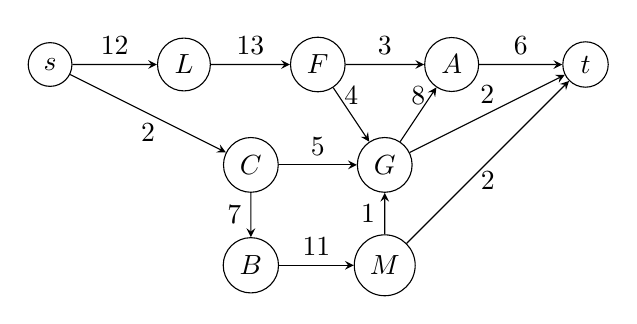
\begin{tikzpicture}[scale=0.85]
			\usetikzlibrary{arrows.meta}
			\node[draw,circle] (v0) at (0,  3.5)	{$s$};
			\node[draw,circle] (v1) at (2,  3.5)    {$L$};
			\node[draw,circle] (v2) at (4,  3.5)	{$F$};
			\node[draw,circle] (v3) at (6,  3.5)    {$A$};
			\node[draw,circle] (v4) at (8,  3.5)	{$t$};
			\node[draw,circle] (v5) at (3,    2)    {$C$};
			\node[draw,circle] (v6) at (5,    2)    {$G$};
			\node[draw,circle] (v7) at (3,  0.5)    {$B$};
			\node[draw,circle] (v8) at (5,  0.5)    {$M$};
			
			\def\list {v0/v1/12, v1/v2/13, v2/v3/3, v3/v4/6, v2/v6/4, v5/v6/5, v6/v3/8,
			v6/v4/2, v7/v8/11}  % list elements
			\foreach \u\v\weight in \list
			{	\draw[-stealth] (\u) -- (\v) node [midway, above] {\weight};
			}
			\def\vertical {v5/v7/7, v8/v6/1 %v0/v4/3, v2/v5/4, v2/v9/4%, v3/v7/7, v6/v10/1, v11/v7/2
            }  % list elements
			\foreach \u\v\weight in \vertical
			{	\draw[-stealth] (\u) -- (\v) node [midway, left] {\weight};
			}
			\def\down {v0/v5/2, v8/v4/2} %list elements
			\foreach \u\v\weight in \down
			{   \draw[-stealth] (\u) -- (\v) node [midway, below] {\weight};
			}
		\end{tikzpicture}
    	\end{minipage}
    	\begin{minipage}[b]{0.5\textwidth}
    		\centering
    		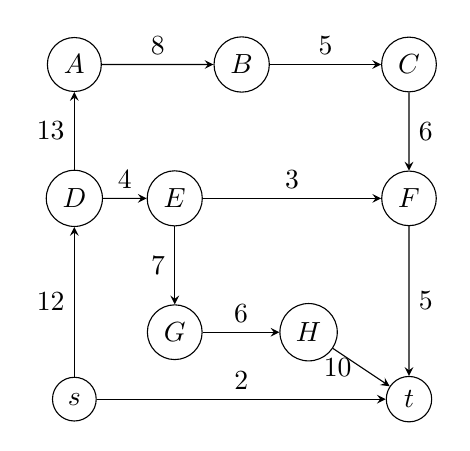
\begin{tikzpicture}[scale=0.85]
			\usetikzlibrary{arrows.meta}
			\node[draw,circle] (v0) at (0  ,    0)	  {$s$};
			\node[draw,circle] (v1) at (0  ,    5)    {$A$};
			\node[draw,circle] (v2) at (2.5,    5)	  {$B$};
			\node[draw,circle] (v3) at (5  ,    5)    {$C$};
			\node[draw,circle] (v4) at (0  ,    3)	  {$D$};
			\node[draw,circle] (v5) at (1.5,    3)    {$E$};
			\node[draw,circle] (v6) at (5  ,    3)    {$F$};
			\node[draw,circle] (v7) at (1.5,    1)    {$G$};
			\node[draw,circle] (v8) at (3.5,    1)    {$H$};
			\node[draw,circle] (v9) at (5  ,    0)    {$t$};
			
			\def\list {v0/v4/12, v4/v1/13, v5/v7/7, v8/v9/10}  % label left from edge
			\foreach \u\v\weight in \list
			{	\draw[-stealth] (\u) -- (\v) node [midway, left] {\weight};
			}
			\def\vertical {v0/v9/2, v1/v2/8, v2/v3/5, v4/v5/4, v5/v6/3, v7/v8/6}  % label above edge
			\foreach \u\v\weight in \vertical
			{	\draw[-stealth] (\u) -- (\v) node [midway, above] {\weight};
			}
			\def\down {v3/v6/6, v6/v9/5} % label right from edge
			\foreach \u\v\weight in \down
			{   \draw[-stealth] (\u) -- (\v) node [midway, right] {\weight};
			}
		\end{tikzpicture}
    	
    	\end{minipage}
    \end{figure}
\end{aufgabe}

\begin{aufgabe}[Blutspende]
    % KT exercise 7.8
    Statistisch steigt die Zahl der Unfälle mit dem Beginn des Frühlings an. Für die steigende Anzahl an Notfällen braucht es auch vermehrt Bluttransfusionen. Stell dir vor, du arbeitest für ein Krankenhaus, das beurteilen muss, ob seine Blutreserven ausreichend sind.\\
    Beim Blutspenden gibt es eine grundlegende Regel: Eine Person hat in ihrem Blut bestimmte Antigene (Du kannst dir Antigene als eine Art molekulare Signatur vorstellen). Bei einer Blutspende kann ein Person nur Blut empfangen, welches die gleichen Antigene hat, wie das eigene. Konkret gesagt unterteilt dieses Prinzip das Blut in vier Gruppen: A, B, AB und O. Blutgruppe A hat das Antigen A, Blutgruppe B hat das Antigen B, Blutgruppe AB hat beide und Blutgruppe O hat keines der Antigene. Demnach können Patienten mit Blutgruppe A nur Blut der Gruppen A und O, Patienten der Blutgruppe B nur Blut der Gruppen B und O, Patienten der Blutgruppe O nur Blut der Gruppe O und Patienten der Gruppe AB Blut aller Blutgruppen empfangen.
    \begin{enumerate}
    	\item Seien $s_O,s_A,s_B$ und $s_{AB}$ der Vorrat der vier Blutgruppen, angegeben in ganzen Einheiten. Nimm an, dass das Krankenhaus den prognostizierten Bedarf $d_O, d_A,d_B$ und $d_{AB}$ an Blut der nächsten Woche kennt. Gib einen Algorithmus an, der in Polynomialzeit ausgibt, ob das vorrätige Blut den prognostizierten Bedarf der nächsten Woche deckt.\\
    	\item Schaue dir das folgende Beispiel an. Das Krankenhaus prognostiziert für die nächste Woche einen Bedarf von maximal $100$ Einheiten an Blut. Die durchschnittliche Verteilung der Blutgruppen über die U.S.-Bevölkerung liegt bei $45\%$ Blutgruppe O, $42\%$ Blutgruppe A, $10\%$ Blutgruppe B und $3\%$ Blutgruppe AB. Das Krankenhaus möchte wissen, ob seine Vorräte ausreichend sind, wenn 100 Patienten mit der erwarteten Verteilung behandelt werden müssen. Es sind $105$ Einheiten an Blut vorrätig. Die Tabelle gibt den Vorrat und die Nachfrage an Blut an.
    	
    	\vspace{4mm}
    	\begin{center}
    	\begin{tabular}{|c|c|c|}
    	\hline 
    	Blutgruppe & Vorrat & Nachfrage \\ 
    	\hline 
    	O & 50 & 45 \\ 
    	\hline 
    	A & 36 & 42 \\ 
    	\hline 
    	B & 11 & 8 \\ 
    	\hline 
    	AB & 8 & 3 \\ 
    	\hline 
    	\end{tabular}
    	\end{center}
    	\vspace{4mm}
    	Sind die 105 vorrätigen Einheiten an Blut ausreichend, um der Nachfrage von 100 Einheiten gerecht zu werden? Finde eine Verteilung, sodass die maximale Anzahl an Patienten behandelt werden kann. Benutze einen minimalen Kapazität-Schnitt, um zu begründen, warum nicht alle Patienten behandelt werden können. Stelle außerdem eine verständliche Erklärung dieses Umstandes für die Krankenhausverwaltung bereit, die ALGO2 nicht belegt haben. (Die Erklärung soll also die Worte \textit{Fluss, Schnitt} oder \textit{Graph} nicht enthalten.
    \end{enumerate}
\end{aufgabe}

\begin{aufgabe}[Weihnachtsbäume]
    % Algorithms and Data Structures 2 - networks2.pdf
    Der Dekan (insert guten Namen) hat dich beauftragt, die jährliche Weihnachtsfeier für alle Student:innen der Goethe-Universität zu organisieren. Du musst einen Plan erstellen, auf dem die Platzierung der Tische im Casino-Festsaal vermerkt ist. Um den Brandschutz zu gewährleisten, hat die Frankfurter Feuerwehr den Festsaal in ein quadratisches $n \times m$ Gitter aufgeteilt und dir mitgeteilt, dass höchstens zwei Tische in jeder Zeile und höchstens ein Tisch in jeder Spalte aufgestellt werden dürfen. Leider liebt der Dekan Weihnachtsbäume und so hat er in vielen Bereichen schon welche aufgestellt. Du kannst keinen Tisch in den selben Bereich stellen, in dem schon ein Weihnachtsbaum steht.
    
    \textbf{Beispiel.} Es gilt $n = 4$ und $m = 8$. Die $\star$ stellen Weihnachtsbäume dar und $T$ die Tische. In diesem Beispiel ist die maximale Anzahl an Tischen, die platziert werden können, 7.
    
    \vspace{4mm}
    \begin{center}
    \begin{tabular}{|c|c|c|c|c|c|c|c|}
    \hline 
    \rule[-1ex]{0pt}{2.5ex} $\star$ & $T$ &  &  &  &  &  & $T$ \\ 
    \hline 
    \rule[-1ex]{0pt}{2.5ex} $T$ & $\star$ & $\star$ & $T$ & $\star$ & $\star$ &  & $\star$ \\ 
    \hline 
    \rule[-1ex]{0pt}{2.5ex}  & $\star$ & $\star$ &  & $\star$ & $\star$ & $T$ & $\star$ \\ 
    \hline 
    \rule[-1ex]{0pt}{2.5ex}  & $\star$ & $T$ & $\star$ &  & $T$ & $\star$ &  \\ 
    \hline 
    \end{tabular} 
    \end{center}
    \vspace{4mm}
    \begin{enumerate}
    	\item Modelliere das Problem als Graphenproblem. Erkläre, wie du das machst und zeichne den zum Beispiel passenden Graphen.\\
    	\item Beschreibe einen Algorithmus, der, gegeben $n,m$ und die Platzierung der Weihnachtsbäume, eine maximale Anzahl an Tischen, die im Festsaal platziert werden können, ausgibt. Analysiere die asymptotische Laufzeit deines Algorithmus. Denke daran, die Korrektheit deines Algorithmus zu zeigen.\\
    	\item Implementiere deinen Algorithmus in Python oder Java.
    \end{enumerate}
\end{aufgabe}

\section*{Donnerstag}

\begin{aufgabe}[Flucht]
    % KT exercise 7.14
\end{aufgabe}

\begin{aufgabe}[Eulerwege in gemischten Graphen]
    % Algorithms and Data Structures 2 - networks2.pdf
\end{aufgabe}

\begin{aufgabe}[Puzzle der Woche: Das Zwölf-Münzen Problem]
	% Algorithms and Data Structures 2 - networks2.pdf
	
\end{aufgabe}

\end{document}
